\tikzstyle{block} = [rectangle, draw, minimum height=1cm, minimum width=1cm]
\tikzstyle{every node}=[font=\LARGE]
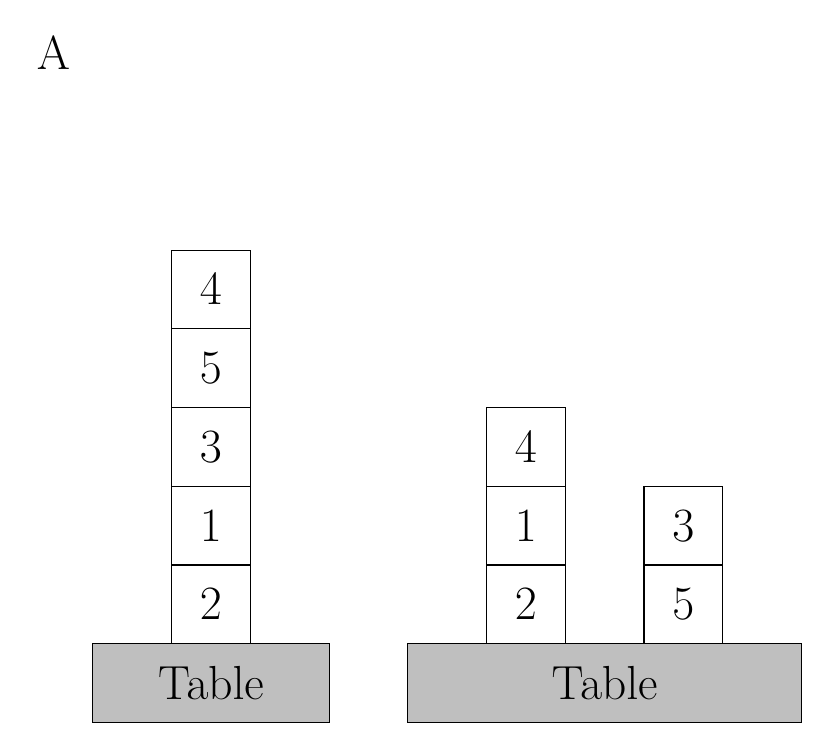
\begin{tikzpicture}[baseline]
	\node[block] at (0,5) {4};
	\node[block] at (0,4) {5};
	\node[block] at (0,3) {3};
	\node[block] at (0,2) {1};
	\node[block] at (0,1) {2};
	\node[rectangle, draw, minimum width=3cm, minimum height=1cm, fill=gray!50] at (0,0) {Table};
	\begin{scope}[xshift=3cm]
		\node[block] at (1,3) {4};
		\node[block] at (1,2) {1};
		\node[block] at (1,1) {2};
		\node[block] at (3,2) {3};
		\node[block] at (3,1) {5};
		\node[rectangle, draw, minimum width=5cm, minimum height=1cm, fill=gray!50] at (2,0) {Table};
	\end{scope}
	\node at (-2,8) {\LARGE A};
\end{tikzpicture}
